\documentclass[tikz,border=10pt]{standalone}
\begin{document}
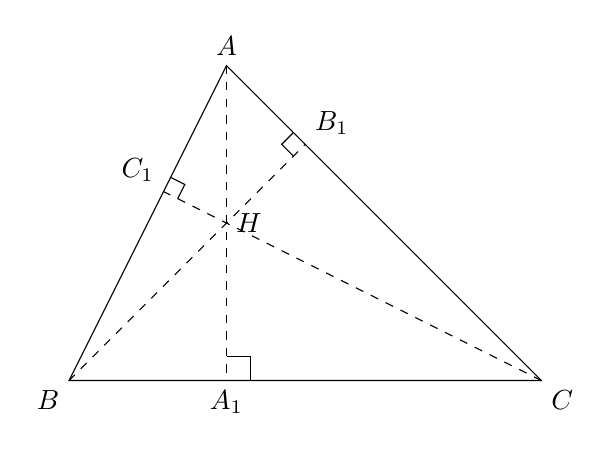
\begin{tikzpicture}
    \coordinate (A) at (2, 4);
    \coordinate (B) at (0, 0);
    \coordinate (C) at (6, 0);
    \coordinate (A1) at (2, 0);
    \coordinate (B1) at (3, 3);
    \coordinate (C1) at (1.2, 2.4);
    \coordinate (H) at (2, 2);

    % Triangle sides (solid)
    \draw (A) -- (B) -- (C) -- cycle;

    % Altitudes (dashed)
    \draw[dashed] (A) -- (A1);
    \draw[dashed] (B) -- (B1);
    \draw[dashed] (C) -- (C1);

    % Right angle marks
    % At A1
    \draw (2, 0.3) -- (2.3, 0.3) -- (2.3, 0);
    % At B1
    \draw (2.85, 2.85) -- (2.7, 3.0) -- (2.85, 3.15);
    % At C1
    \draw (1.38, 2.31) -- (1.47, 2.49) -- (1.29, 2.58);

    % Labels
    \node[above] at (A) {$A$};
    \node[below left] at (B) {$B$};
    \node[below right] at (C) {$C$};
    \node[below] at (A1) {$A_1$};
    \node[above right] at (B1) {$B_1$};
    \node[above left] at (C1) {$C_1$};
    \node[right] at (H) {$H$};
\end{tikzpicture}
\end{document}
